\begin{frame}
    \frametitle{Planned Stage II-3: ROLLO Single Objective Problems}
    \begin{itemize}
        \item Center-peaking fuel density is nonideal for other key reactor core 
        qualities, such as maximal heat transfer and minimal power peaking factor (PPF).
        Thus, the AHTR slab optimization problem must be extended to include 
        these key reactor core qualities. 
    \end{itemize}
    \begin{block}{Objectives}
        \vspace{-0.2cm}
    \begin{table}
        \caption{ROLLO optimization problem objectives with their quantification 
        descriptions.}
        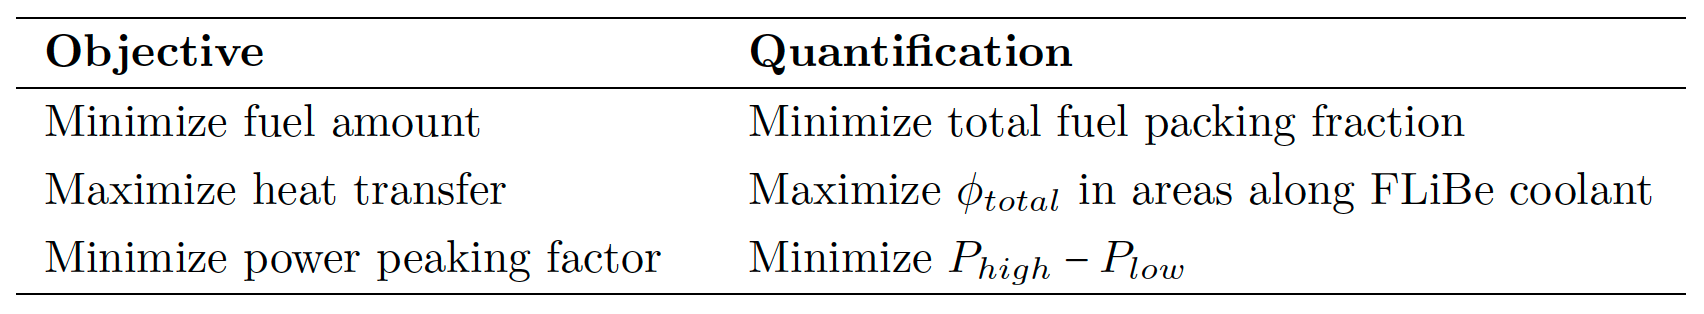
\includegraphics[width=0.7\linewidth]{figures/opt-obj.png}
    \end{table}
\end{block}
\vspace{-0.5cm}
\begin{block}{Control Parameters}
    \begin{itemize}
        \item TRISO particle packing fraction distribution $\rho_{TRISO}(\vec{r})$
        \item Total fuel packing fraction
        \item FLiBe coolant channel shape 
    \end{itemize}
\end{block}
\end{frame}

\begin{frame}
    \frametitle{Planned Stage II-3: ROLLO Single Objective Problems}
    \begin{table}
        \caption{Proposed ROLLO simulations for AHTR fuel assembly single 
        objective optimization.
        PF: Total Fuel Packing Fraction, $\dot{Q}$: Heat transfer, $PPF$: Power Peaking Factor, 
        $\rho_{TRISO}(\vec{r})$: \gls{TRISO} particle distribution}
        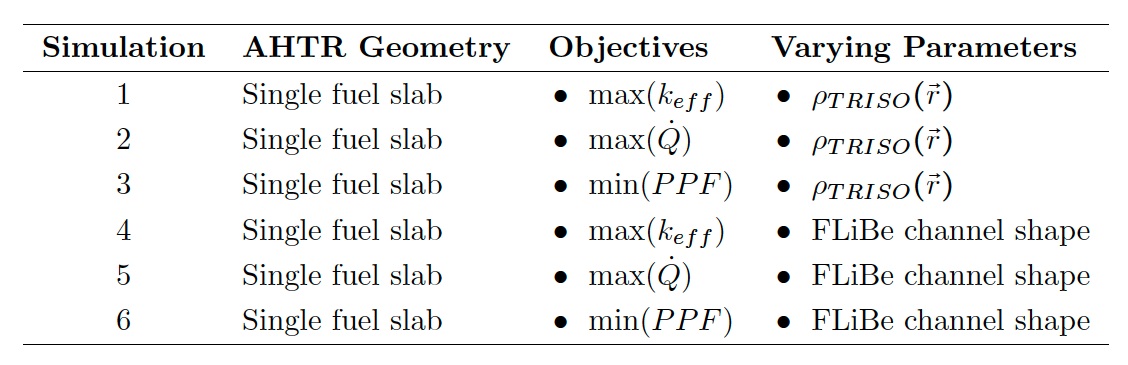
\includegraphics[width=0.8\linewidth]{figures/single-obj.png}
    \end{table}
\end{frame}